\documentclass[a4paper, 11pt]{article}
\usepackage[margin=3cm]{geometry}
\usepackage[]{fontenc}
\usepackage[utf8]{inputenc}
\usepackage[italian]{babel}
\usepackage{geometry}
\geometry{a4paper, top=2cm, bottom=3cm, left=1.5cm, right=1.5cm, heightrounded, bindingoffset=5mm}
\usepackage{amsmath}
\usepackage{amssymb}
\usepackage{gensymb}
\usepackage{graphicx}
\usepackage{psfrag,amsmath,amsfonts,verbatim}
\usepackage{xcolor}
\usepackage{color,soul}
\usepackage{fancyhdr}
\usepackage{indentfirst}
\usepackage{graphicx}
\usepackage{newlfont}
\usepackage{amssymb}
\usepackage{amsmath}
\usepackage{latexsym}
\usepackage{amsthm}
%\usepackage{subfigure}
\usepackage{subcaption}
\usepackage{psfrag}
\usepackage{footnote}
\usepackage{graphics}
\usepackage{color}
\usepackage{hyperref}
\usepackage{tikz}


\usetikzlibrary{snakes}
\usetikzlibrary{positioning}
\usetikzlibrary{shapes,arrows}

	
	\tikzstyle{block} = [draw, fill=white, rectangle, 
	minimum height=3em, minimum width=6em]
	\tikzstyle{sum} = [draw, fill=white, circle, node distance=1cm]
	\tikzstyle{input} = [coordinate]
	\tikzstyle{output} = [coordinate]
	\tikzstyle{pinstyle} = [pin edge={to-,thin,black}]

\newcommand{\courseacronym}{CAT}
\newcommand{\coursename}{Controlli Automatici - T}
\newcommand{\tipology}{\dots}
\newcommand{\trace}{\dots}
\newcommand{\projectname}{Nome del Progetto}
\newcommand{\group}{\dots}

%opening
\title{ \vspace{-1in}
		\huge \strut \coursename \strut 
		\\
		\Large  \strut Progetto Tipologia \tipology - Traccia \trace 
		\\
		\Large  \strut \projectname\strut
		\\
		\Large  \strut Gruppo \group\strut
		\vspace{-0.4cm}
}
\author{Autore, \dots}
\date{}

\begin{document}

\maketitle
\vspace{-0.5cm}

Il progetto riguarda il controllo di \dots, la cui dinamica viene descritta dalle seguenti equazioni differenziali 
%
\begin{subequations}\label{eq:system}
\begin{align}
	\dots,
\end{align}
\end{subequations}
%
dove \dots rappresenta \dots.


\section{Espressione del sistema in forma di stato e calcolo del sistema linearizzato intorno ad una coppia di equilibrio}

Innanzitutto, esprimiamo il sistema~\eqref{eq:system} nella seguente forma di stato
%
\begin{subequations}
\begin{align}\label{eq:state_form}
	\dot{x} &= f(x,u)
	\\
	y &= h(x,u).
\end{align}
\end{subequations}
%
Pertanto, andiamo individuare lo stato $x$, l'ingresso $u$ e l'uscita $y$ del sistema come segue 
%
\begin{align*}
	x := \dots, \quad u := \dots, \quad y := \dots.
\end{align*}
%
Coerentemente con questa scelta, ricaviamo dal sistema~\eqref{eq:system} la seguente espressione per le funzioni $f$ ed $h$
%
\begin{align*}
	f(x,u) &:= \dots
	\\
	h(x,u) &:= \dots.
\end{align*}
%
Una volta calcolate $f$ ed $h$ esprimiamo~\eqref{eq:system} nella seguente forma di stato
%
\begin{subequations}\label{eq:our_system_state_form}
\begin{align}
	\begin{bmatrix}
		\dot{x}_1
		\\
		\dots
	\end{bmatrix} &= \dots \label{eq:state_form_1}
	\\
	y &= \dots.
\end{align}
\end{subequations}
%
Per trovare la coppia di equilibrio $(x_e, u_e)$ di~\eqref{eq:our_system_state_form}, andiamo a risolvere il seguente sistema di equazioni
%
\begin{align}
	\dots,
\end{align}
%
dal quale otteniamo
%
\begin{align}
	x_e := \dots,  \quad u_e = \dots.\label{eq:equilibirum_pair}
\end{align}
%
Definiamo le variabili alle variazioni $\delta x$, $\delta u$ e $\delta y$ come 
%
\begin{align*}
	\delta x &= \dots, 
	\quad
	\delta u = \dots, 
	\quad
	\delta y = \dots.
\end{align*}
%
L'evoluzione del sistema espressa nelle variabili alle variazioni pu\`o essere approssimativamente descritta mediante il seguente sistema lineare
%
\begin{subequations}\label{eq:linearized_system}
\begin{align}
	\delta \dot{x} &= A\delta x + B\delta u
	\\
	\delta y &= C\delta x + D\delta u,
\end{align}
\end{subequations}
%
dove le matrici $A$, $B$, $C$ e $D$ vengono calcolate come
%
\begin{subequations}\label{eq:matrices}
\begin{align}
	A &= \dots
	\\
	B &= \dots
	\\
	C &= \dots
	\\
	D &= \dots.
\end{align}
\end{subequations}
%
\section{Calcolo Funzione di Trasferimento}

In questa sezione, andiamo a calcolare la funzione di trasferimento $G(s)$ dall'ingresso $\delta u$ all'uscita $\delta y$ mediante la seguente formula 
%
%
\begin{align}\label{eq:transfer_function}
G(s) = \dots = \dots.
\end{align}
%
Dunque il sistema linearizzato~\eqref{eq:linearized_system} è caratterizzato dalla funzione di trasferimento~\eqref{eq:transfer_function} con $\dots$ poli $p_1 = \cdots, \cdots$ e $\dots$ zeri $z_i =\cdots$. In Figura \dots mostriamo il corrispondente diagramma di Bode. 

\dots

\section{Mappatura specifiche del regolatore}
\label{sec:specifications}

Le specifiche da soddisfare sono
\begin{itemize}
	\item[1)] \dots\\
	\item[2)] \dots\\
	....\\
	\item[6)] \dots.
\end{itemize}
%
Andiamo ad effettuare la mappatura punto per punto le specifiche richieste. \dots  

Pertanto, in Figura \dots, mostriamo il diagramma di Bode della funzione di trasferimento $G(s)$ con le zone proibite emerse dalla mappatura delle specifiche.

\dots

\section{Sintesi del regolatore statico}
\label{sec:static_regulator}

In questa sezione progettiamo il regolatore statico $R_s(s)$ partendo dalle analisi fatte in sezione~\ref{sec:specifications}.

\dots

Dunque, definiamo la funzione estesa $G_e(s) = R_s(s)G(s)$ e, in Figura \dots, mostriamo il suo diagramma di Bode per verificare se e quali zone proibite vengono attraversate.

\dots

Da Figura \dots, emerge \dots


\section{Sintesi del regolatore dinamico}
\label{sec:dynamic_regulator}

In questa sezione, progettiamo il regolatore dinamico $R_d(s)$. 
%
Dalle analisi fatte in Sezione~\ref{sec:static_regulator}, notiamo di essere nello Scenario di tipo \dots. Dunque, progettiamo $R_d(s)$ ricorrendo a \dots


In Figura \dots, mostriamo il diagramma di Bode della funzione d'anello $L(s) = R_d(s) G_e(s)$

\dots

\section{Test sul sistema linearizzato}

In questa sezione, testiamo l'efficacia del controllore progettato sul sistema linearizzato con $w(t) = 1(t)$, $d(t)=\sum_{k = 1}^{4} \sin(5\space\cdot\space 10^{4}kt)  $.

In Figura \ref{fig:step_response}, si mostra la risposta del sistema linearizzato ad un gradino unitario. \`E possibile notare come essa rispetti le specifiche richieste riguardanti tempo di assestamento, sovraelongazione e massimo errore a regime.
 
\begin{figure}[h!]
	\centering
	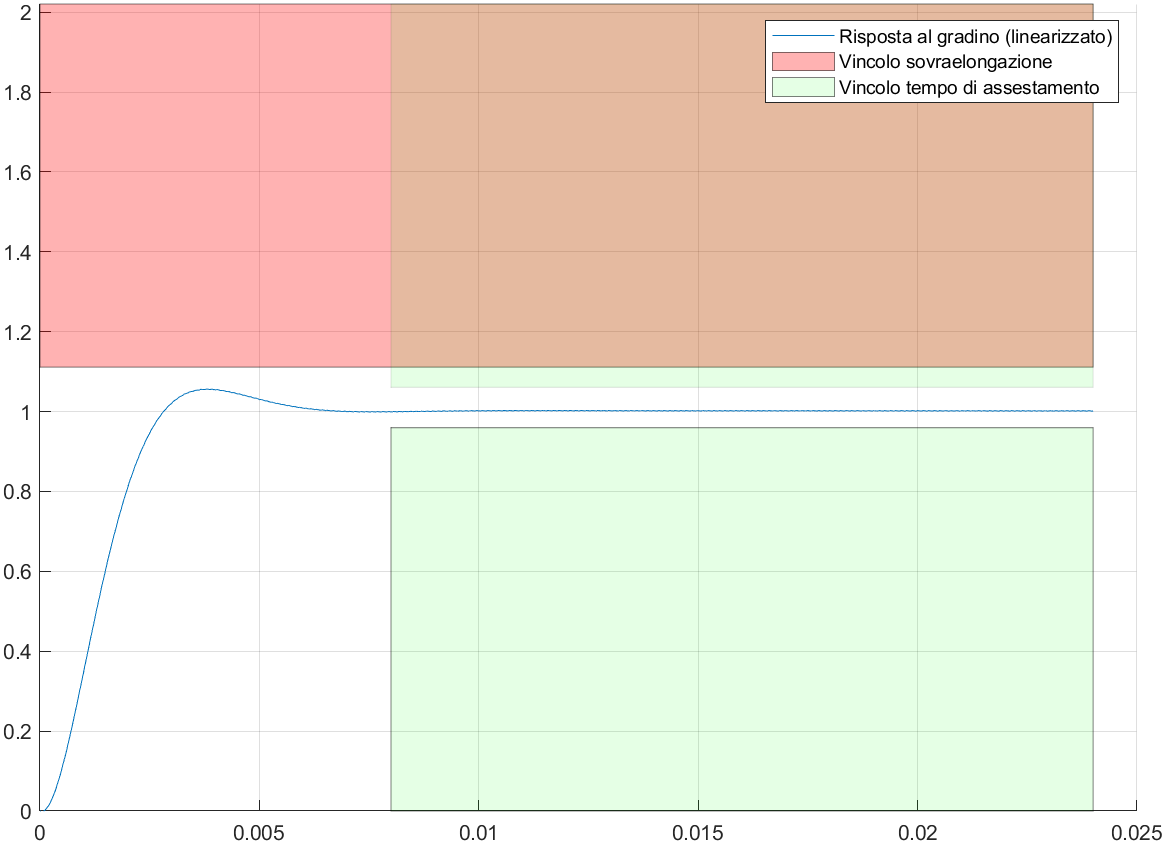
\includegraphics[width=0.8\linewidth]{C:/Users/loren/Desktop/CAT-Immagini/stepRespLin.png}
	\caption{Risposta del sistema linearizzato ad un gradino unitario.}
	\label{fig:step_response}
\end{figure}

Questo risultato \`e stato ottenuto progettando un regolatore statico $R_s(s)$ adeguato al fine di mantenere l'errore a regime inferiore a $0.004$ (come spiegato nella Sezione~\ref{sec:static_regulator}) 
e un regolatore dinamico $R_d(s)$ che facesse s\`i che il sistema rispettasse un vincolo sul margine di fase $M_f$ tale per cui si evitino sovraelongazione e tempo di assestamento superiori alle specifiche richieste
(come spiegato nella Sezione~\ref{sec:dynamic_regulator}).

\section{Test sul sistema non lineare}

In questa sezione, testiamo l'efficacia del controllore progettato sul modello non lineare con \dots


\section{Punti opzionali}

\subsection{Primo punto}

\dots 

\subsection{Secondo punto}

\dots

\subsection{Terzo punto}

\dots

\section{Conclusioni}

\dots

\end{document}
